\documentclass[conference]{IEEEtran}

\usepackage[T1]{fontenc}
\usepackage[utf8]{inputenc}

\usepackage{amsmath}
\usepackage{booktabs}
\usepackage{cite}
\usepackage{graphicx}
\usepackage[hidelinks]{hyperref}
\graphicspath{{figures/}}
\title{Fruit-Fly Nerve-Cord Wiring and Motor Drive in a Simulated Hexapod}
\author{\IEEEauthorblockN{Puneeth Pradeep}
\IEEEauthorblockA{High School Student\\
\textit{Nolensville High School}\\
Nolensville, TN, USA\\
puneethp2009@gmail.com}}
\hypersetup{pdftitle={Fruit-Fly Nerve-Cord Wiring and Motor Drive in a Simulated Hexapod},pdfauthor={Puneeth Pradeep}}
\begin{document}
\maketitle

\begin{abstract}
A connectome records connections between nerve cells. We test whether fruit-fly nerve-cord wiring changes forward drive (signed forward displacement over an 8 s episode) in a simulated non-fly hexapod without training. We build a MaleCNS v1.0 model with 11,000 nodes and 485,074 signed connections. A fixed, hand-written map converts 260 motor channels into 18 joint targets. The map and model settings remain fixed across comparisons. Four fixed, untrained readout experiments (A--D) test lesions, rewiring, body variation, and named-input contrasts; Experiment E adds a separate hand-written rhythm generator for a descriptive CPG-assisted walking test. Removing outgoing connections from second-thoracic-segment neurons reduces forward drive by 0.01120 m in all 20 episodes ($p_{\mathrm{holm}} = 1.9 \times 10^{-6}$). Removing sensory-pathway edges changes forward drive by less than $10^{-8}$ m. Forward drive declines overall across six rewiring fractions (Spearman $\rho = -0.886$). Across nine body-test comparisons covering seven unique settings and three repeated baseline cases, measured wiring produces positive forward drive; shuffled-weight control means remain negative, and none of the 12 control seeds matches or exceeds it. Named descending inputs produce motor-pool cosine distances of 0.612 to 0.723 with measured wiring, compared with 0.038 to 0.097 after rewiring. A separate hand-written rhythm generator produces 0.839 m of CPG-assisted walking in 8 s without falling. Shuffling network timing reduces net forward displacement to 0.442 m, below the 0.765 m from the generator alone. These results concern wiring effects under this fixed map and model; connectome-alone walking is not tested.
\end{abstract}
\begin{IEEEkeywords}
connectome, Drosophila, ventral nerve cord, hexapod, motor control, simulation
\end{IEEEkeywords}

\section{Introduction}
In the fruit fly, or \textit{Drosophila}, the ventral nerve cord (VNC) links brain commands and body feedback to motor output~\cite{takemura2024manc,cheong2026premotor}. We use this circuit to test how measured connections affect movement. The wiring map alone cannot answer this question: movement also depends on neural activity, the body, and the interface between them.

The MaleCNS dataset provides public connection and annotation data for an adult male fly's brain and nerve cord~\cite{malecns}. We use the released graph to ask whether measured wiring leaves a measurable signal under a fixed, untrained motor map. Its annotations identify cell types and associated body regions~\cite{marin2024annotation}. We select cells and connections from this dataset to build the network model. We then connect its motor output to a simulated body and measure the resulting movement.

Previous studies have connected nervous-system models to artificial bodies. A \textit{C.\ elegans} connectome model produced movement in a wheeled robot~\cite{valencia2023robot}. A fruit-fly model combines a whole-brain connectome, a fly-shaped body, and trained components~\cite{jin2026flygm}. Other studies keep the network fixed but learn a readout from its activity~\cite{damicelli2022reservoir,suarez2024conn2res}. We ask what measured wiring contributes when neither the network nor its motor map is trained.

We connect a fruit-fly nerve-cord model to a simulated non-fly hexapod (Fig.~\ref{fig:overview}). Its leg shapes and joints differ from a fly's, so we use a fixed map to convert motor activity into robot-joint targets. We compare measured wiring with matched controls using the same body and interface. Neither the connections nor the map is trained. This is a conditional test of one graph under one fixed cross-species map, not a claim that fruit-fly wiring generally controls locomotion.

We ask four questions: which connections affect forward drive, how drive changes with rewiring, whether the comparison holds across body variations, and whether named inputs produce distinct motor-pool activity. Experiments A--C address the first three questions, and Experiment D addresses the fourth using the labeled-line approach in whole-brain fly simulation~\cite{jin2026flygm}. Experiment E is an additional descriptive test of CPG-assisted walking.

\begin{figure*}[t]
\centering
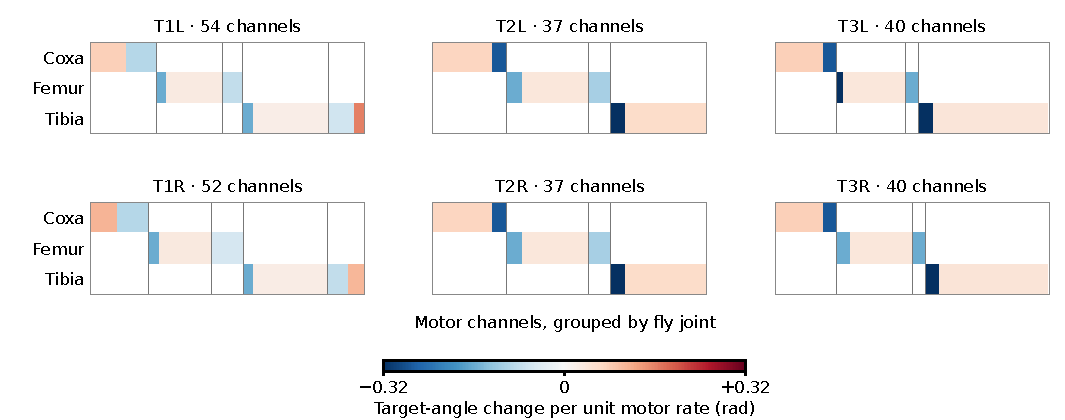
\includegraphics[width=\textwidth]{fixed_motor_map.pdf}
\caption{Fixed map from 260 motor channels to 18 joint targets. Panels show front (T1), middle (T2), and rear (T3) legs, left (L) above right (R); rows are coxa, femur, and tibia from top to bottom. Color gives the target-angle coefficient, not synaptic sign; white is zero. Cross-leg coefficients are zero and omitted. Motor rate is normalized to the fixed 250 Hz ceiling.}
\label{fig:motor-map}
\end{figure*}

\section{Methodology}
\subsection{Building the Nerve-Cord Model}
We build the network from the official MaleCNS v1.0 connection and annotation files~\cite{malecns}. Published cell labels identify candidate leg-coordination neurons in the three thoracic regions, T1, T2, and T3~\cite{cheong2026premotor}. Our selection includes 212 cells across 62 of 66 labels. Four labels are absent or outside the selection. The 212 annotated cells form the selected seed set. Adding their connected upstream cells provides paths from incoming commands to motor output and gives a final network with 11,000 model nodes and 260 motor-output channels.

We use synapse counts as connection strengths and exclude connections with fewer than five synapses. We assign positive signs to acetylcholine connections and negative signs to gamma-aminobutyric acid (GABA) and glutamate connections. Connections without a selected sign are excluded. This leaves 485,074 signed connections. The signs are modeling assumptions, not a complete description of each synapse's biological effect.

Each node follows the leaky integrate-and-fire formulation from whole-brain fly simulation~\cite{jin2026flygm}. The model accumulates input in a membrane potential and emits discrete spikes. We stimulate named descending inputs with Poisson input at the stated rate. For each fixed-map comparison, the named input set, Poisson rate, and 8 s readout window are held fixed across network conditions; Experiment D varies named input sets and uses 50, 100, 150, and 200 Hz. Activity decays over time, and motor firing rates are normalized by a fixed ceiling of 250 Hz. We keep connection weights and activity settings fixed across comparisons. We fix the synaptic weight at $w_{\mathrm{syn}} = 0.275$ mV per synapse. All other constants are taken from published electrophysiology: resting and reset potential $-52$ mV, threshold $-45$ mV, membrane time scale 20 ms, synaptic time constant 5 ms, refractory period 2.2 ms, and synaptic delay 1.8 ms. Synaptic weight is $w_{\mathrm{syn}}$ times the signed synapse count. The integrator uses exponential-Euler at a 2 ms substep under a 20 ms control step. The substep sets spike-time resolution rather than stability, and the 1.8 ms synaptic delay is quantised to one substep. Poisson drive is thinned onto the substep grid as one Bernoulli draw per substep at $p = r\,\Delta t$. The refractory period bounds a neuron at 454.5 Hz in continuous time, but a discrete integrator holds it out for whole substeps only, giving the 250 Hz ceiling used to normalize motor rates. These settings remain fixed across comparisons.


\subsection{The Two Interfaces}
We use two interfaces to separate motor drive from walking.

The \emph{fixed-map interface} converts motor rates into 18 joint targets without body feedback. We specified this map from anatomical pool labels before measuring forward drive and kept it unchanged across comparisons. Results therefore concern this map, not all possible maps. The interface adds no rhythm. We measure signed forward displacement over an 8 s episode and report it in metres below; we call this quantity forward drive. Experiments A through C use this interface. Experiment D instead reads the 260 motor channels directly for selectivity analysis.

For each fly leg and joint group, we subtract the mean extensor-like activity from the mean flexor-like activity. The robot coxa uses the fly coxa pool; the robot femur averages the available trochanter and femur pools; the robot tibia averages the available tibia and tarsus pools. Fixed gains of $(-0.55, 0.65, 0.65)$ convert these scores into offsets from the home pose. Figure~\ref{fig:motor-map} shows the resulting coefficients. Each channel affects only its assigned leg and robot joint; the map does not create coordination between legs.

\begin{figure*}[t]
\centering
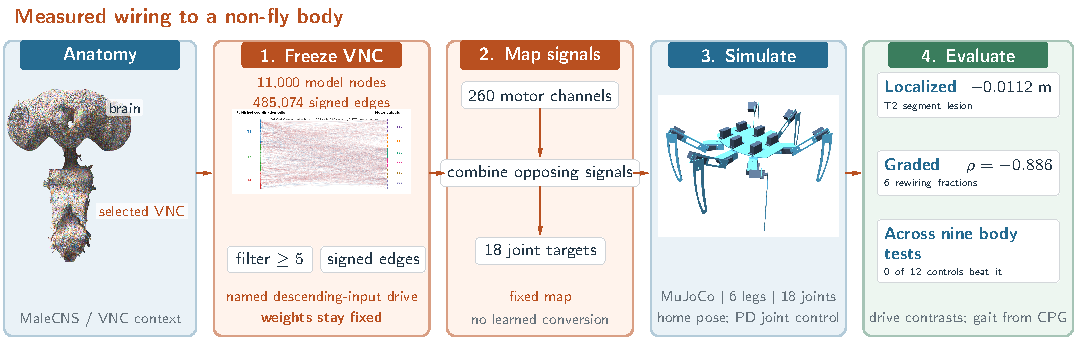
\includegraphics[width=0.98\textwidth]{overview_pipeline.pdf}
\caption{Fixed-map pipeline: selected VNC network, motor map, simulated body, evaluation. The nine body tests are robustness cases over seven unique settings; three nominal baseline rows reuse the same body. Anatomy: Janelia FlyEM and collaborators, CC BY 4.0~\cite{malecns}, VNC pivoted for visibility.}
\label{fig:overview}
\end{figure*}

The \emph{CPG-coupled interface} adds a hand-written central pattern generator. Its rhythm generator is based on published fly gait work~\cite{chun2021tripod}. Network output modulates this rhythm. The generator supplies rhythm and inter-leg coordination. We therefore report Experiment E as a descriptive test of CPG-assisted network modulation, not of connectome-alone walking.

We simulate the body in MuJoCo~\cite{todorov2012mujoco}. Figure~\ref{fig:platform} shows its geometry. Within each comparison, the graph, body, motor map, interface, and episode starts are held fixed; Experiment C changes body settings between comparisons. The 20 episodes per condition are simulator repeats with shared random starts. Each control seed creates one rewiring or weight-shuffle randomization of the same graph; it is not an independent graph or body. The phase analysis in Experiment D uses 30 Poisson realizations. Sign-flip tests use the shared episode starts in Experiment A and control seeds in Experiment C. Thus intervals and p-values describe sampled episode or control-seed variation conditional on one graph, body, map, and fixed settings; they do not quantify uncertainty over those design choices. Holm correction covers two lesions in Experiment A and nine body tests in Experiment C.

\begin{figure}[t]
\centering
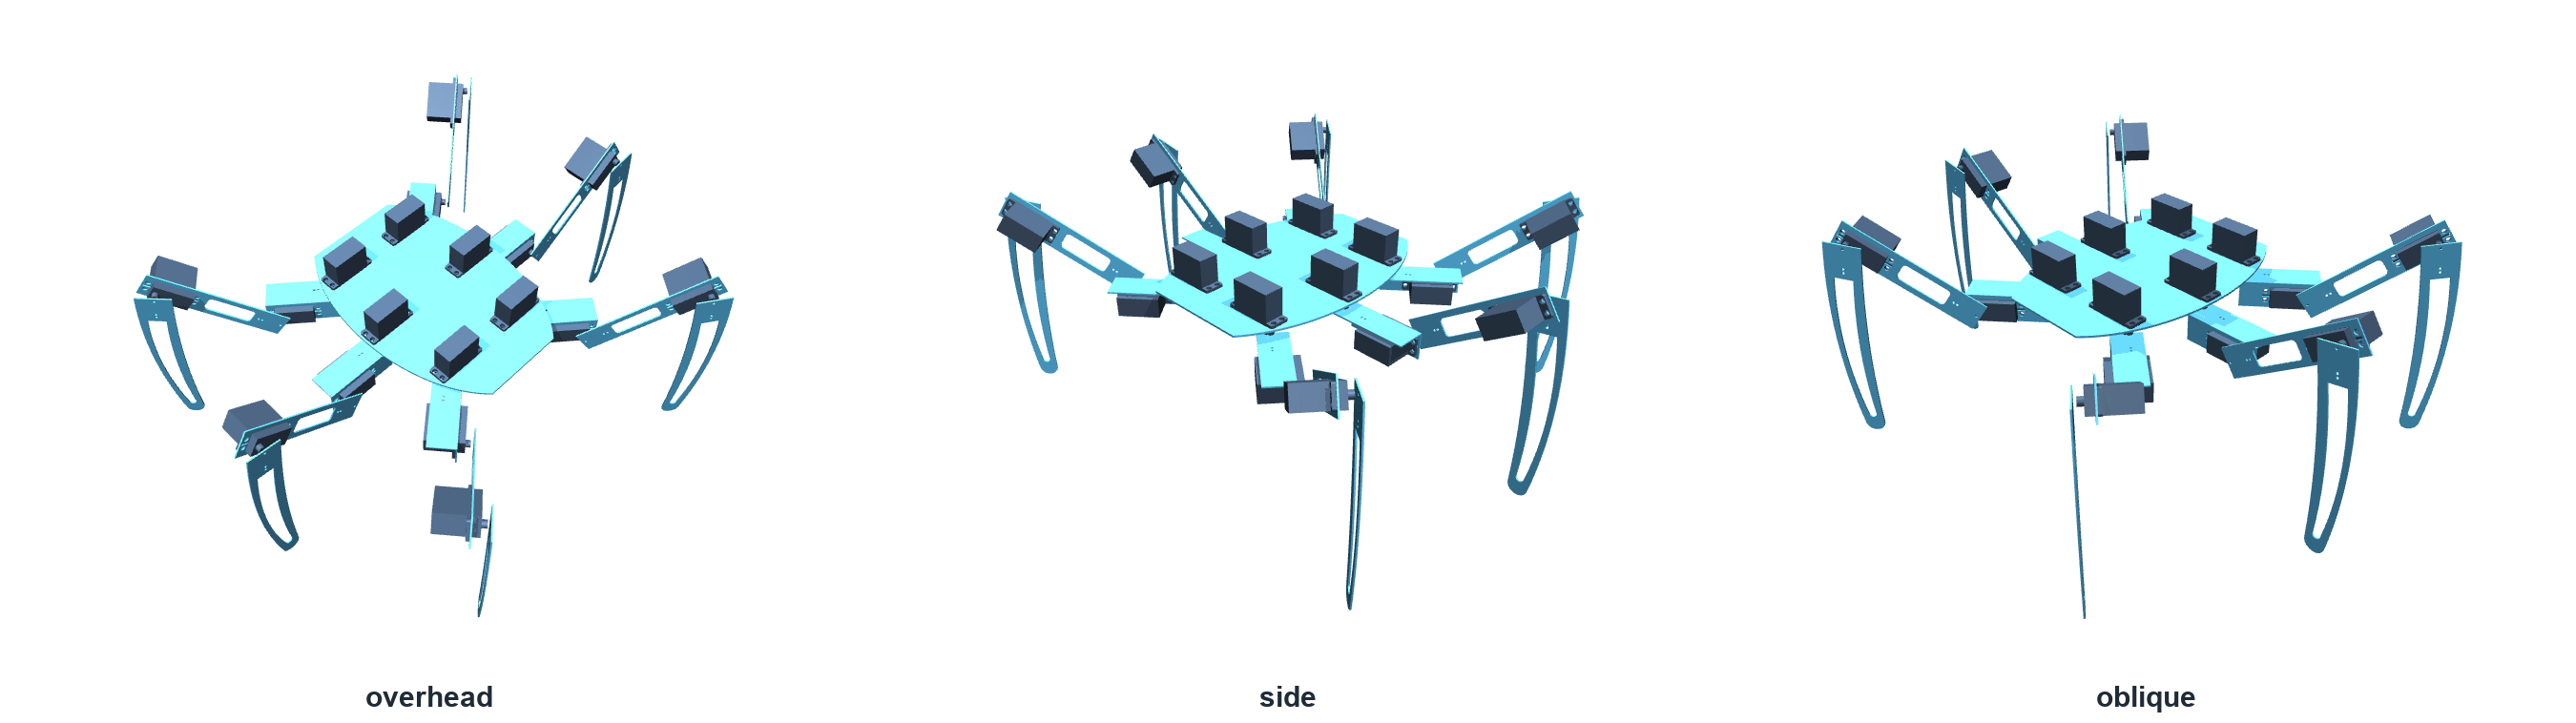
\includegraphics[width=\columnwidth]{platform_views.png}
\caption{Simulated hexapod in its home pose: six legs, 18 actuated joints.}
\label{fig:platform}
\end{figure}

\subsection{Controls}
We use matched controls to test connection patterns and weight assignments separately. The \emph{rewired} control swaps edge endpoints while preserving each node's incoming and outgoing connection counts and the multiset of weights. The \emph{shuffled-weight} control moves signed weights among existing connections without changing their endpoints. The rewired comparison can therefore change both topology and edge-weight placement; it does not isolate topology alone. Before evaluating movement, we center each control history on its own channel mean and rescale it so each of the 18 joint-target channels matches the measured network's temporal standard deviation. This matching controls marginal channel scale only; it does not match cross-channel covariance, phase, target bounds, or delivered torque. We apply the same rule to every control before evaluating forward drive, and the match uses temporal variation rather than the movement outcome.

\begin{table}[t]
\caption{Main settings for the fixed-interface experiments.}
\label{tab:settings}
\centering
\scriptsize
\begin{tabular}{@{}ll@{}}
\toprule
Component & Setting\\
\midrule
Measured network & 11,000 nodes; 485,074 connections\\
Motor channels & 260\\
Robot joints & 18 (6 legs)\\
Episode length & 8 s\\
Episodes per condition & 20 (simulator repeats; shared starts)\\
Control seeds & 12 rewired; 12 shuffled-weight (independent)\\
Rate ceiling & 250 Hz\\
Parameter updates & 0 (no training)\\
\bottomrule
\end{tabular}
\end{table}

\section{Experiments and Results}

\subsection{Experiment A: Connection Lesions}
We test whether removing annotated connection groups changes forward drive by removing outgoing connections from neurons with a given region or pathway annotation. We then rerun the fixed-map interface using the same 20 episode starts. The lesions target different connection groups; they are not matched in size.

Removing outgoing connections from T2 neurons reduces forward drive from $+0.00208$ m to $-0.00912$ m. T2 is the second thoracic segment and serves the middle pair of legs. The loss is $0.01120$ m, with a bootstrap confidence interval of $[0.01100, 0.01140]$. All 20 episodes show a loss. An exact one-sided sign-flip test over shared starts gives $p_{\mathrm{holm}} = 1.9 \times 10^{-6}$. Removing sensory-pathway connections changes forward drive by less than $10^{-8}$ m ($p_{\mathrm{holm}} = 1$). This small change is consistent with an interface that receives no body feedback.

The lesions remove 134,858 and 26,187 connections, respectively. Their unequal sizes prevent us from attributing the contrast to location alone; the result concerns the tested T2-associated edge set rather than T2 location in isolation. Section~V discusses this limitation.

\subsection{Experiment B: Rewiring}
We test whether forward drive changes as more measured connections are rewired, rather than comparing only intact and fully rewired graphs. Degree-preserving swaps use six fractions, $\alpha \in \{0, 0.1, 0.25, 0.5, 0.75, 1.0\}$. Each nonzero fraction uses 12 independent seeds and 20 episodes per seed.

Forward drive falls from $+0.00208$ m at $\alpha = 0$ to $-0.00480$ m at $\alpha = 1.0$. The overall trend is negative, but not strictly monotonic: Spearman $\rho = -0.886$ (Table~\ref{tab:dose}). The measured graph's mean is above the upper confidence limit at every nonzero fraction. This six-point trend is descriptive and associates greater rewiring with lower forward drive under the fixed map.

\begin{table}[t]
\caption{Dose response. Forward drive against the fraction of the graph rewired by degree-preserving swaps. Twelve independent seeds per nonzero fraction, 20 simulator episodes each. The measured graph at $\alpha=0$ has no rewiring seed.}
\label{tab:dose}
\centering
\small
\begin{tabular}{@{}lrr@{}}
\toprule
Rewired fraction $\alpha$ & Forward drive (m) & 95\% CI (m)\\
\midrule
0.00 (measured) & $+0.00208$ & $[+0.00151, +0.00269]$\\
0.10 & $-0.00164$ & $[-0.00338, +0.00030]$\\
0.25 & $-0.00077$ & $[-0.00315, +0.00188]$\\
0.50 & $-0.00378$ & $[-0.00586, -0.00163]$\\
0.75 & $-0.00490$ & $[-0.00735, -0.00269]$\\
1.00 & $-0.00480$ & $[-0.00655, -0.00303]$\\
\midrule
\multicolumn{3}{@{}l}{Spearman $\rho = -0.886$}\\
\bottomrule
\end{tabular}
\end{table}

\subsection{Experiment C: Body Variations}
We test whether the network comparison depends on one body configuration. We vary leg length, body mass, and ground friction at three settings each, giving nine tests across seven unique body settings, since the three nominal rows repeat the same baseline body. These repeated baseline rows are robustness cases, not independent body configurations. Each test compares measured wiring with 12 shuffled-weight seeds.

Measured wiring produces positive forward drive in all nine tests, from $+0.00070$ m to $+0.00488$ m. Shuffled-weight control means remain negative, ranging from $-0.00216$ m to $-0.00496$ m. None of the 12 control seeds matches or exceeds the measured network in any variation. An exact one-sided sign-flip test over the 12 control seeds gives $p_{\mathrm{holm}} = 0.0022$ for each variation (Table~\ref{tab:body}). The measured-minus-control contrast was positive at each tested setting.

\begin{table}[t]
\caption{Body variation tests. Forward drive under nine body-test comparisons over seven unique settings, measured network against 12 shuffled-weight seeds. The three $\times1.00$ rows reuse the same baseline body. ``Beat'' counts control seeds matching or exceeding the measured network.}
\label{tab:body}
\centering
\scriptsize
\begin{tabular}{@{}lrrr@{}}
\toprule
Body variation & Measured (m) & Control mean (m) & Beat\\
\midrule
Leg length $\times 0.85$ & $+0.00346$ & $-0.00307$ & 0/12\\
Leg length $\times 1.00$ & $+0.00208$ & $-0.00366$ & 0/12\\
Leg length $\times 1.15$ & $+0.00092$ & $-0.00496$ & 0/12\\
Body mass $\times 0.85$ & $+0.00488$ & $-0.00475$ & 0/12\\
Body mass $\times 1.00$ & $+0.00208$ & $-0.00366$ & 0/12\\
Body mass $\times 1.15$ & $+0.00070$ & $-0.00322$ & 0/12\\
Friction $\times 0.70$ & $+0.00208$ & $-0.00366$ & 0/12\\
Friction $\times 1.00$ & $+0.00208$ & $-0.00366$ & 0/12\\
Friction $\times 1.30$ & $+0.00138$ & $-0.00216$ & 0/12\\
\midrule
\multicolumn{4}{@{}l}{$p_{\mathrm{holm}} = 0.0022$ for every variation}\\
\bottomrule
\end{tabular}
\end{table}

\subsection{Experiment D: Named Inputs}
The labeled-line test asks whether named descending inputs produce distinct motor-pool activity, following whole-brain fly simulation~\cite{jin2026flygm}. We stimulate each named input set at four Poisson rates and read the 260 motor channels. Cosine distance between z-scored motor-pool rows measures separation between the resulting activity patterns; larger values indicate more separation. The primary contrasts are DNg100 versus all descending inputs and DNg100 versus its left-side subset. Before this comparison, we excluded DNb08 because its output entered a second rising regime near the end of the 30 s window. We declared this exclusion before the comparison and retained all measured rows.

The DNg100-versus-all-descending contrast gives distances of 0.612 to 0.723 with measured wiring across four rates. Distances are 0.038 to 0.097 after rewiring and 0.191 to 0.632 after weight shuffling (Table~\ref{tab:sel}). The DNg100-versus-left-side-subset contrast gives a measured-network distance of 0.031 at 50 Hz and 0.134 at 200 Hz; the rewired control rises from 0.003 to 0.016. In six of eight contrasts, the measured network exceeds both controls by more than the measured network's standard deviation across 30 Poisson realizations. These are descriptive comparisons, not independent-seed tests.

We also measure the relative timing of opposing motor pools in 20 retained leg-by-joint cells (Fig.~\ref{fig:phase}); undefined cells are not counted as inside the target band. The displayed 150-Hz summary labels 3 of 20 cells inside the target band. Across 30 Poisson realizations, the measured mean count is 4.00 (SD 0.91); the rewired and shuffled-weight controls have mean counts of 0.040 and 0.056, respectively. We use 12 of 20 as a descriptive threshold for this exploratory readout. The measured network is below that threshold, so the phase criterion was not met.

\begin{figure}[t]
\centering
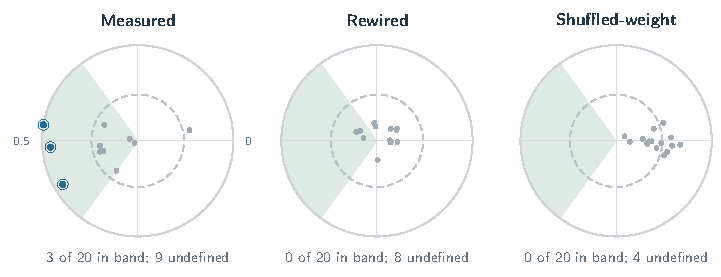
\includegraphics[width=\columnwidth]{phase_circle.pdf}
\caption{Opposing motor-pool timing in 20 cells under DNg100 drive at 150 Hz. The displayed summary labels 3 of 20 cells inside the target band; across 30 Poisson realizations, the count averages 4.00 (SD 0.91). Angle is phase difference, and radius is concentration. Rings mark cells inside the target wedge ($0.5 \pm 0.15$ cycles) above 0.3 concentration. Shuffled weights give higher mean concentration (0.208 vs.\ 0.185), but near synchrony rather than the target phase.}
\label{fig:phase}
\end{figure}

\begin{table}[t]
\caption{Labeled-line selectivity. Cosine distance between z-scored motor-pool rows for DNg100 versus all descending inputs and DNg100 versus its left-side subset. Values are descriptive summaries for the listed rates.}
\label{tab:sel}
\centering
\scriptsize
\begin{tabular}{@{}lrrr@{}}
\toprule
Contrast and rate & Measured & Rewired & \shortstack{Shuffled-\\weight}\\
\midrule
All descending, 50 Hz & 0.723 & 0.038 & 0.632\\
All descending, 100 Hz & 0.644 & 0.063 & 0.437\\
All descending, 150 Hz & 0.612 & 0.081 & 0.220\\
All descending, 200 Hz & 0.632 & 0.097 & 0.191\\
\midrule
Left subset, 50 Hz & 0.031 & 0.003 & 0.382\\
Left subset, 100 Hz & 0.076 & 0.008 & 0.311\\
Left subset, 150 Hz & 0.109 & 0.013 & 0.093\\
Left subset, 200 Hz & 0.134 & 0.016 & 0.054\\
\bottomrule
\end{tabular}
\end{table}

\subsection{Experiment E: CPG-assisted walking}
With the hand-written rhythm generator, the model produces CPG-assisted walking with net forward displacement of 0.839 m in 8 s, a path-to-forward ratio of 2.46, and no falls across 20 simulator episodes (Fig.~\ref{fig:walk}). The path-to-forward ratio is total path length divided by net forward displacement. The generator-only condition produces net forward displacement of 0.765 m. The difference is $+0.074$ m, smaller than the network condition's across-realization standard deviation of 0.408 m. These values do not show a walking-distance benefit from the connectome.

Shuffling network output along the time axis changes the outcome. We hold the rhythm generator, amplitude, body, and episode starts fixed. Net forward displacement falls to 0.442 m, below the 0.765 m from the generator-only condition. We treat this timing-shuffle comparison as descriptive evidence of an interaction, not as a separate walking-performance test.

\begin{figure}[t]
\centering
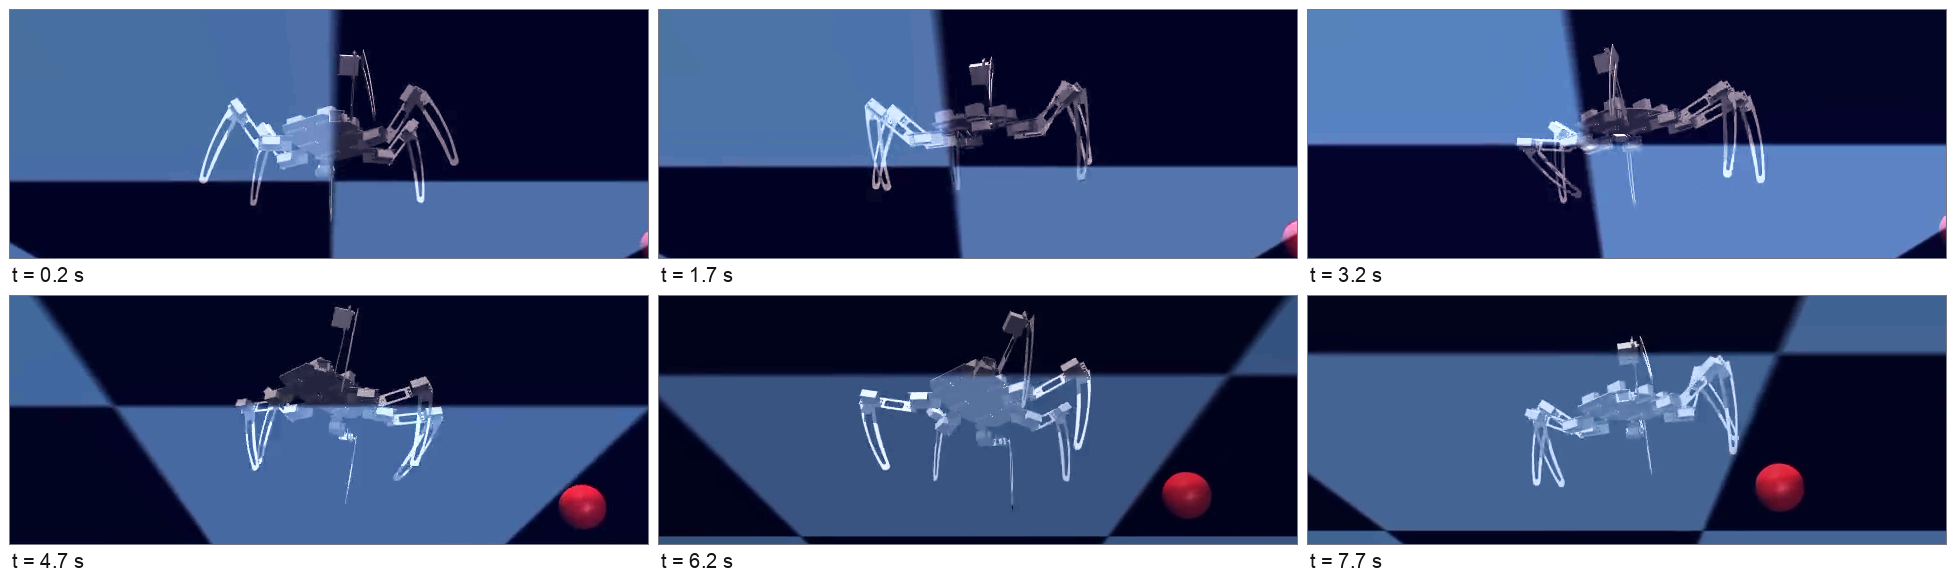
\includegraphics[width=\columnwidth]{walk_filmstrip.png}
\caption{One representative 8 s rollout covering 0.798 m, sampled every 1.5 s; the 20-episode mean is 0.839 m. Alternating tripod postures in MuJoCo~\cite{todorov2012mujoco}; the red marker tracks forward travel.}
\label{fig:walk}
\end{figure}

\section{Discussion}
Measured wiring affects motor drive under the fixed interface. T2 removal reduces forward drive; sensory-pathway removal does not. Forward drive also declines overall with rewiring, and measured wiring remains ahead of all 12 shuffled-weight controls across nine body-test comparisons. These results support a wiring-dependent effect under the fixed map and model assumptions, but do not isolate lesion location from lesion size.

For the all-descending contrasts, rewiring preserves connection counts but reduces the measured distance by approximately 6.5 to 19.0 fold across the four rates. Weight shuffling preserves the connection pattern and exceeds measured wiring on two of eight selectivity contrasts. The measured network did not lead on every contrast, so these descriptive results do not support a general advantage for its weight values.

The walking result should be read as an interaction test: the generator supplies rhythm and inter-leg coordination. The distance difference from the generator-only condition is small relative to the reported variation. The experiment does not test gait generated by the connectome alone. Time shuffling reduces travel below the generator-only condition, suggesting an interaction between network timing and the supplied rhythm; this comparison is descriptive.

\section{Limitations}
Three limitations shape the interpretation.

Experiment A removes 134,858 connections for T2 and 26,187 for the sensory pathway. The effects differ, but lesion size may explain part of that difference. T1 and T3 lesions would remove 102,353 and 111,131 connections, respectively. We did not run these comparisons; they would help test whether the effect is specific to T2.

The antagonist-phase readout reaches 4.00 of 20 cells, below the 12-cell threshold. The DNb08 exclusion described in Section~III-D narrows the primary named-input comparison because its output entered a second rising regime near the end of the 30 s window. This behavior is consistent with runaway saturation, not a stable labeled-line response.

The fixed map receives no proprioceptive feedback about the body's state, so it remains open-loop. Its small, millimetre-scale displacement measures forward drive, not sustained locomotion. Synaptic signs are inferred from neurotransmitter labels under a modeling assumption. The motor map is one possible conversion under this assumption.

\section{Conclusion}
We connected a frozen fruit-fly nerve-cord model to a simulated non-fly hexapod without training. Under the fixed map and model assumptions, measured wiring affects forward drive across lesion, rewiring, and nine body-test comparisons covering seven unique settings. Named-input contrasts produce more distinct motor-pool activity than the rewired control, but not uniformly more than the shuffled-weight control, and the phase criterion is not met. Walking relies on the added rhythm generator, and the distance comparison does not establish a benefit from the network; connectome-alone gait was not tested. Body feedback and footfall measurements are needed to test whether the motor-drive effect extends to gait.

\renewcommand{\IEEEbibitemsep}{0pt plus 0pt}
\bibliographystyle{IEEEtran}
\bibliography{flycraft_bibm_draft}

\end{document}
